\chapter{Introduction}
\label{cap:introduction}

The focus of this research is on finding modes of Sum-Product Networks with Gaussian leaves, which are compact representations of Gaussian Mixture Models. This introductory chapter presents the motivation and rationale for this study (Section \ref{sec:motivation}), describes the objectives and methodology (Section \ref{sec:methodology}), summarizes the contributions (Section \ref{sec:contributions}), and outlines the structure of the document (Section \ref{sec:organization}).

\section{Motivation}
\label{sec:motivation}

Sum-Product Networks \citep[SPNs;][]{Poon2011} are a relatively recent class of expressive statistical models, that exploit the use of arithmetic circuits \citep{Darwiche2003, Rooshenas2014} to efficiently represent complicated probability distributions.

Their graphical structure encodes context-specific independence among random variables (RVs), which makes them a form of probabilistic graphical models \citep[PGMs;][]{Koller2009}. However, SPNs differ from other PGMs from an important computational perspective: unlike Bayesian Networks and Markov Networks, exact marginal and conditional probability inference in SPNs is tractable, taking linear time with respect to the size of the network.

SPNs share similarities with neural networks, as they are defined by a directed acyclic computation graph in which each node computes a function of its input \citep{Hsu2017}. However, there are important differences between SPNs and other neural networks. For example, the structure of an SPN naturally delivers a principled probabilistic representation where each sub-network represents a joint distribution, and standard probabilistic operations such as marginalization and conditioning can be efficiently derived by message-passing through the structure. Moreover, SPNs can be learned online \citep{Lee2013, Jaini2016} and in a distributed fashion \citep{Rashwan2016}.

The ability to capture a rich set of independences and produce reliable and fast inference has rendered SPNs a competitive approach for many challenging machine learning tasks \citep{Poon2011, Llerena2017, Peharz2014, Cheng2014, Amer2016}.

Although SPNs can be defined over discrete or continuous RVs, most works to date focus on SPNs over categorical RVs. In spite of that, many real-world applications are better modeled by continuous variables \citep{Jaini2016}. While marginal inference works the same way for discrete and continuous SPNs (except that discrete SPNs compute probability masses, whereas continuous SPNs compute densities), certain algorithms that operate on discrete SPNs do not function with continuous SPNs and vice versa.

The focus of this study is on a specific class of continuous SPNs named Gaussian SPNs (GSPNs), which have Gaussian distributions at their leaves. GSPNs are efficient representations of Gaussian Mixture Models (GMMs) with numerous components. Specifically, they encode GMMs with a number of components that is exponential on the size of the network.

GMMs themselves are an expressive class of models for density estimation, widely applied in both statistics and machine learning. GMMs are convex combinations of Gaussian densities and inherit some of the advantages of them, such as being analytically tractable for many computations. However, even with few components they exhibit a quite complex behavior. In fact, the family of Gaussian mixtures is a universal approximator for continuous densities \citep{Titterington1985}. To our knowledge, the relation between GSPNs and GMMs has been so far unexplored in the literature, and, in particular, there is no prior research that links techniques for locating modes of GMMs to those of GSPNs.

The problem of finding maxima (modes) of Gaussian mixtures has been long studied. Despite this, it remains a challenging problem to identify the number of modes that a mixture of $k$ Gaussians in $d$ dimensions can have \citep{Amendola2019}. The most commonly used techniques for finding modes involve hill-climbing algorithms from several points such as Mean-Shift \citep{Fukunaga1975, Carreira-Perpinan2015} and Gradient Ascent \citep{Murphy2012}. To the extent of our knowledge, there are no prior works discussing modes in the context of SPNs.

Finding modes has many applications, and this work focuses on two of them: Maximum-A-Posteriori (MAP) inference and cluster analysis.

MAP inference, the problem of finding the most probable values for a set of variables according to a probability distribution, is a valuable tool for a variety of tasks, particularly those involving data reconstruction. An example of such application is image completion, as demonstrated in Figure \ref{fig:imagecompletion}, which depicts the results of completing the left halves of unseen faces using various algorithms \citep{Poon2011}. The first row dislpays the original images, the second row shows results obtained by MAP inference in an SPN, and the remaining rows show results obtained by other methods (from top to bottom: deep Boltzmann machines, deep belief networks, principal component analysis, and nearest neighbor).

\begin{figure}
  \centering
  \scalebox{0.23}{
    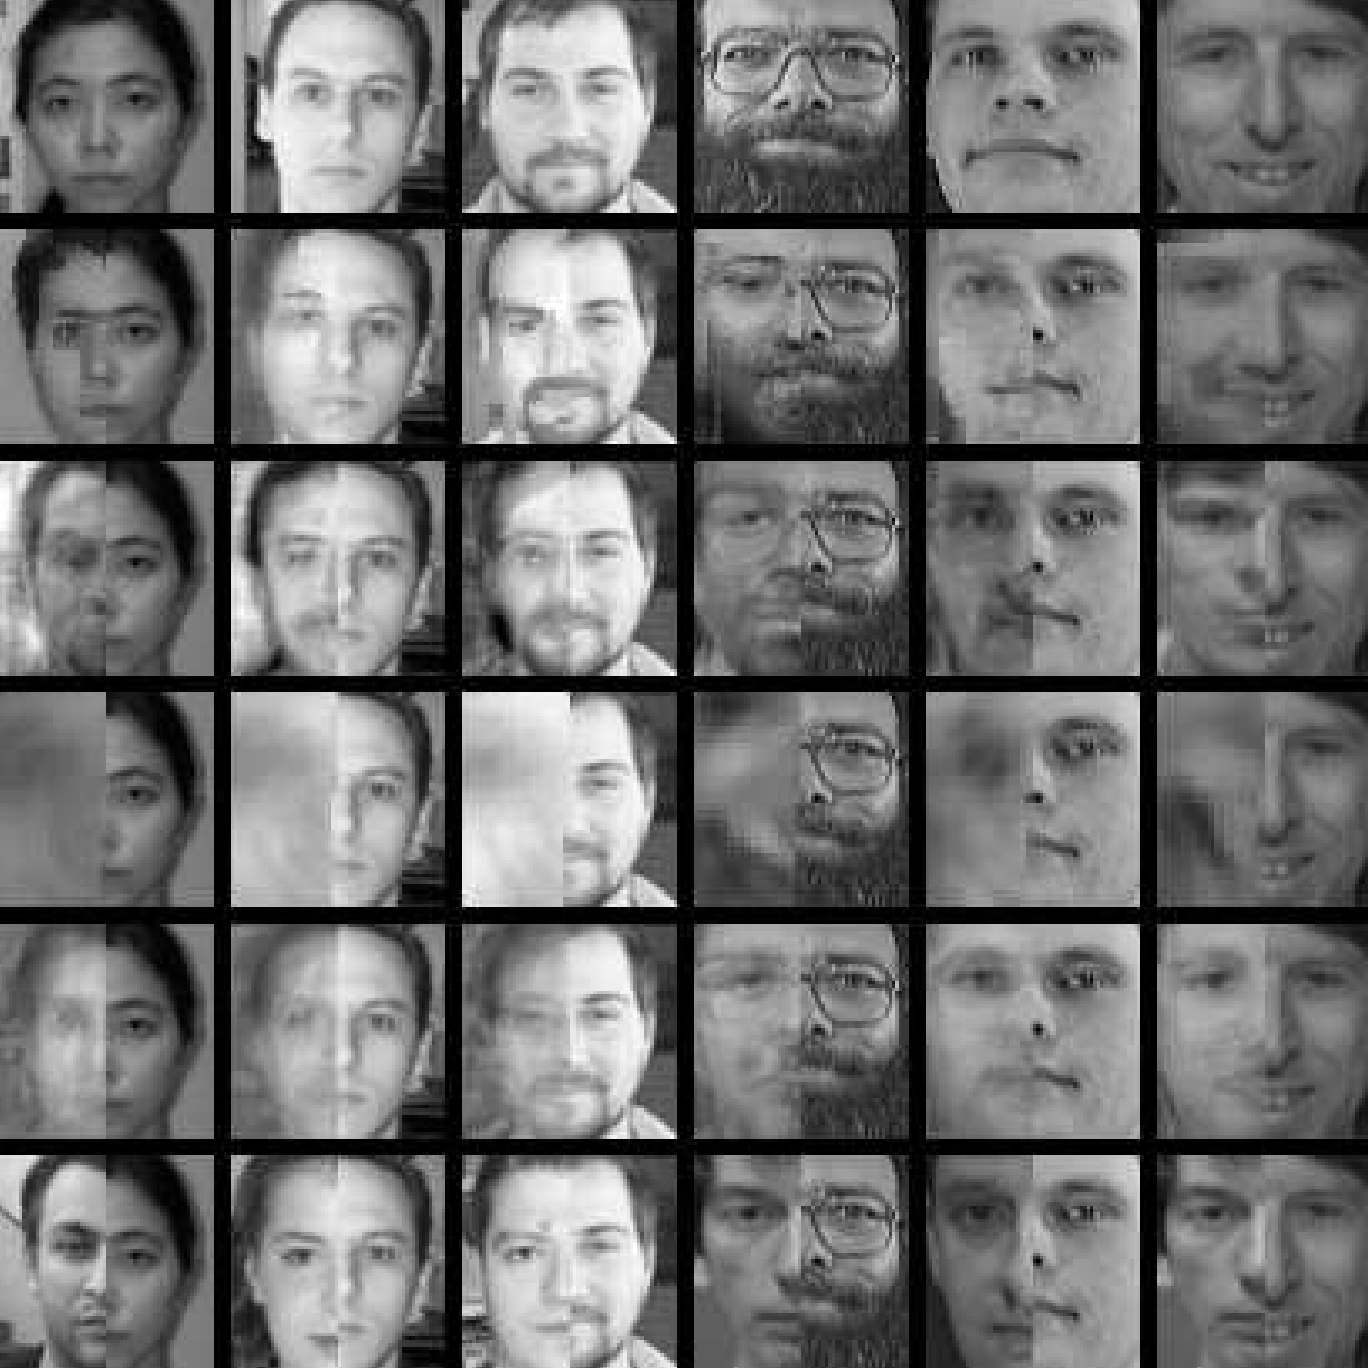
\includegraphics{figures/imagecompletion.png}
  }

  \caption[Sample face completions]{Sample face completions. Source: \citet{Poon2011}.}
  \label{fig:imagecompletion}
\end{figure}

Due to the $\mathcal{NP}$-Hardness of MAP inference in SPNs, various greedy approximation algorithms have been proposed, along with, more recently, some exact methods. However, these approaches have primarily focused on discrete SPNs, with only a few being extendable to continuous domains. Moreover, their experiments have not included continuous data. Finally, these methods typically search only for points corresponding to the modes of a specific component of the mixture, resulting in solutions of uncertain quality that are unable to guarantee even local optimality. Finding the modes of an SPN can help finding solutions to MAP inference.

Regarding cluster analysis, clustering can be approached by considering a density that represents the distribution of data in a given problem, and then taking its modes as representative of clusters. This approach has been successful in several applications; one example is image segmentation \citep{Cheng1995, Comaniciu2002, Li2007}.

We believe that finding modes of GSPNs can allow performing modal clustering with a class of densities that is more expressive and efficient than GMMs. Additionally, clustering is a valuable method for model analysis and model compression.

\section{Goal and methodology}
\label{sec:methodology}

Our goal is to develop a framework for locating modes of Gaussian Sum-Product Networks.

To achieve this, we will examine the connection between GSPNs and GMMs, survey literature concerning the modes of such models, and explore approaches for detecting them. We will propose an algorithm that adapts an EM-style fixed-point iteration method, known as Modal EM, to identify local maxima of GSPNs.

To validate our algorithm, we will carry out experiments on clustering.

\section{Contributions}
\label{sec:contributions}

The main contribution of this work is Modal EM for GSPNs, an algorithm designed to find modes of densities represented by Gaussian Sum-Product Networks. While this contribution has already been published during the author's postgraduate studies in proceedings of a conference \citep{Madeira2022}, this work offers a more comprehensive description of the algorithm and provides a formal proof of its correctness. In addition, we observe the relationship between Modal EM, a fixed-point iterative schema proposed by \citet{Carreira-Perpinan2000} and Mean-Shift. Furthermore, this thesis provides more context about the problem and reports additional experimental results. A paper about modal clustering with GSPNs containing some of the experiments of image segmentation reported in this document has been published in a workshop \citep{Madeira2023}.

\section{Organization}
\label{sec:organization}

The remaining chapters of this document are structured as follows.

Chapter \ref{cap:gmm} provides an overview of Gaussian Mixture Models and establishes the probability notations used throughout the thesis. We also review the literature related to the number of modes of GMMs and the techniques for mode-finding.

Chapter \ref{cap:spn} introduces Sum-Product Networks and explains how they are used for probabilistic reasoning. We discuss their relationship with mixture models, common methods to learning them from data, and the literature on Maximum-A-Posteriori (MAP) inference in discrete SPNs, which is closely related to finding the global maximum of the model.

Chapter \ref{cap:algorithm} details Modal EM for GSPNs, which is an adaptation of a method for locating maxima of GMMs to find modes of GSPNs. We describe the construction of the algorithm, prove its correctness and runtime complexity, and discuss some applications.

Chapter \ref{cap:experiments} presents experimental results obtained by using Modal EM for GSPNs in the aforementioned applications.

Finally, Chapter \ref{cap:final} concludes the work, provides some final thoughts and ideas for future research.
